% buildcmd: latexmk main.tex
\documentclass{article}
\usepackage[titletoc,title]{appendix}
\usepackage{hyperref}
\usepackage{amssymb}
\usepackage{graphicx}
\graphicspath{ {./images/} }
\title{Internationale Physik Olympiade 2023}
\author{Valentin Zwerschke}
\date{September, 2022}

\begin{document}
\maketitle
\section*{Aufgabe 1}
\subsection*{Teilaufgabe a) - Brennweite der Linse}
Zur Bestimmung der Brennweite verwende ich die Linsengleichung
\begin{center}
	$\frac{1}{f}=\frac{1}{g}+\frac{1}{b}$
\end{center}
beziehungsweise nach f aufgelöst
\begin{center}
	$f=\frac{gb}{g+b}=\frac{140cm\cdot16,8cm}{16,8cm+140cm}=\textbf{15cm}$
\end{center}
\subsection*{Teilaufgabe b) - Planparallele Platte zw. Linse und Schirm}
Beim Durchgang eines Lichtstrahls durch eine planparallele Platte wird der Strahl beim Eintritt in das optisch dichtere
Medium zur optischen Achse hin gebrochen und beim Austritt wieder weg von der optischen Achse. Dies geschieht im gleichen Winkel, 
sodass der Strahl insgesamt parallel zum Eingangsstrahl verschoben herauskommt.   
Um qualitativ zu ermitteln, was beim Einsetzen der planparellelen Platte passiert, habe ich die Veränderungen der drei Strahlen (Mittelpunktstrahl, Brennpunktstrahl und Pararllelstrahl) betrachtet.
Der Brennpunktstrahl kommt nach der Linse parallel zur optischen Achse heraus und geht ungebrochen durch die Platte. Die beiden anderen Strahlen werden parallel verschoben und zwar je weiter je größer der Einfallswinkel ist. 
Die verschobenen Strahlen (in rot) schneiden sich hinter der aktuellen Bildebene. Der Schirm muss also nach hinten geschoben werden.
\begin{center}
	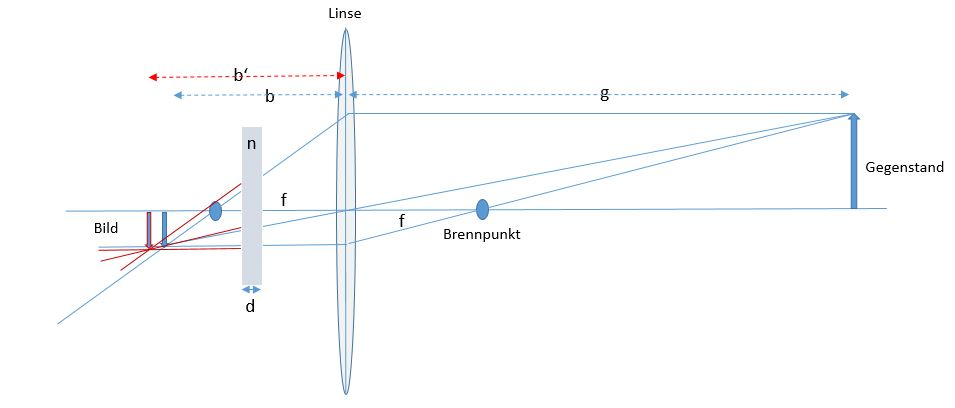
\includegraphics[scale=0.45]{Linse.JPG}
\end{center}

\subsection*{Teilaufgabe c) - Notwendige Verschiebung des Schirms}
Aus dem Brechungsgesetz 
\begin{center}
	$\frac{\sin\alpha}{\sin\beta}=\frac{n_2}{n_1}$
\end{center}
wobei $n_1$ und $n_2$ die Brechungsindizes der beiden Medien sind, $\alpha$ der Einfallswinkel gemessen zur 
optischen Achse und $\beta$ der Austrittswinkel nach dem Übergang ist, 
kann man die Parallelverschiebung zwischen Eingangs- und Ausgangsstrahls beim Durchgang durch die Planparallelel Platte mit einfachen geometrischen Beziehungen berechnen.
Aus Lehrbüchern (oder auch bei \href{https://www.youtube.com/watch?v=j2ptt32nMWg}{Youtube}) findet man die entsprechende Beziehung für die Größe der Verschiebung $s$:
\begin{center}
	$s=d\cdot \sin\alpha \left( 1-\frac{\cos\alpha}{\sqrt{n^2-\sin^2\alpha}}\right)$
\end{center}
Der Einfachheit halber haben wir für die Luft $n=1$ angenommen und den Brechungsindex der 
Platte mit $n$ bezeichnet. Die Dicke der Platte ist $d$ und $\alpha$ der Einfallswinkel eines Strahls. 
Um die notwendige Verschiebung zu berechnen, betrachte ich das folgende Dreieck
\begin{center}
	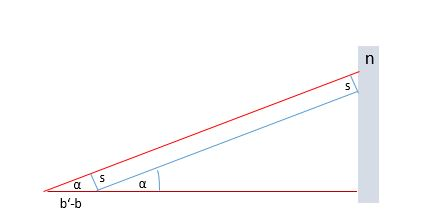
\includegraphics[scale=0.6]{Linse2.JPG}
\end{center}
Es gilt $sin\alpha=s/(b'-b)$ bzw. umgestellt nach der gesuchten Größe $b'-b$
\begin{center}
	$b'-b = \frac{s}{sin\alpha} = d\cdot \sin\alpha \left( 1-\frac{\cos\alpha}{\sqrt{n^2-\sin^2\alpha}}\right) / \sin\alpha $ \\
	$= d \cdot  \left( 1-\frac{\cos\alpha}{\sqrt{n^2-\sin^2\alpha}}\right) \approx d\cdot (1-1/n)$
\end{center}
wobei die letzte Näherung für kleine Winkel $\alpha$ gilt, wovon wir ja ausgehen durften.
Setzt man nun die Werte für $d$ und $n$ aus der Aufgabenstellung ein, so erhält man einen Wert von \textbf{1cm} für die notwendige Verschiebung. 

\section*{Aufgabe 2}
\subsection*{Teilaufgabe a)}
\subsubsection*{1. Epizentrum lokalisieren}
Die Wellen, primär und sekundär, breiten sich kreisförmig vom Epizentrum her aus. Andersherum betrachtet, kann das Signal an einem der Messstellen von jedem Punkt auf einem Kreis mit dem Radius $r$ liegen, 
der sich aus den Messzeiten der Ankunft Primär- und Sekundärwelle berechnen läßt. 
Das Epizentrum sollte im Schnittpunkt der jeweiligen Kreise um die Messstellen liegen. 
Zunächst berechne ich den Zusammenhang zwischen Radius und Ankuftszeitpunkten. 
Es gelten für die Radien der Primär- und Sekundärwellen die Formeln: 
\begin{center}
	$r_{p} = v_p \cdot t_1 = 5,5 km/s \cdot t_1$ \\ 
	$r_{s} = v_s \cdot t_2 = 3,3 km/s \cdot t_2$.
\end{center}
Hier bei ist $t_1$ die Laufzeit der Primärwelle und $t_2$ die Laufzeit der Sekundärwelle.\\
Die beiden Radien sollten gleich groß sein. Mit Hilfe des Gleichsetzungsverfahrens bekommt man die Gleichung: 
\space \space $v_p \cdot t_1  = v_s \cdot t_2$.\\
Anders geschrieben: $0 = (v_p-v_s) \cdot t_1  - v_s \cdot \Delta t$, 
wobei $\Delta t = t_2- t_1$ die Zeitdifferenz zwischen den zwei Signalen ist. 
Löst man nach $t_1$ auf, so bekommt man die Gleichung:
\begin{center}
	\item $t_1 = \frac{v_s }{v_p - v_s}\cdot \Delta t$ 
\end{center}
Aus dieser ergibt sich die gesuchte Beziehung zwischen dem Radius und $\Delta t$. 
\begin{center}
	\item $r = v_p \cdot t_1 = \frac{v_s}{v_p - v_s} \cdot v_p \cdot \Delta t$
\end{center}
Um das Epizentrum herauszubekommen, muss man mit Hilfe eines Zirkels jeweils einen Kreis mit dem entsprechenden Radius um die Messstelle zeichnen. 
Dann sieht man das Epizentrum an dem Schnittpunkt der vier Kreise (vgl. M1 A1). 
Wir benötigen die jeweiligen $\Delta t$ der Stationen. Dazu müssen wir die Differenz zwischen der P- und S-Wellensignalen berechnen.
\begin{itemize}
	\item MIYKNA: $\Delta t \approx 22,85s$ 
	\item ROKUGO: $\Delta t \approx 29,35s$ 
	\item N.KKWH: $\Delta t \approx 17,2s$ 
	\item N.KAKH: $\Delta t \approx 17,3s$ 
\end{itemize}
Als nächstes berechnen wir die jeweiligen Radien: 
\begin{itemize}
	\item $r_M = \frac{3,3km/s}{5,5 km/s - 3,3 km/s} \cdot 5,5 km/s \cdot 22,85 s = 188,5 km$
	\item $r_R = 242,1km$
	\item $r_{N.KK} = 141,9km$
	\item $r_{N.KA} = 142,7km$
\end{itemize}
Nun haben wir alle Radien und tragen die Kreise in die Karte um die Messstationen ein. 
Bei meiner Zeichnung (vgl. M1 A1) schneiden sich die Kreise bei 38,9° Nord, 142,9° Ost. Ungefähr dort sollte das Epizentrum gelegen haben. 
\begin{center}
	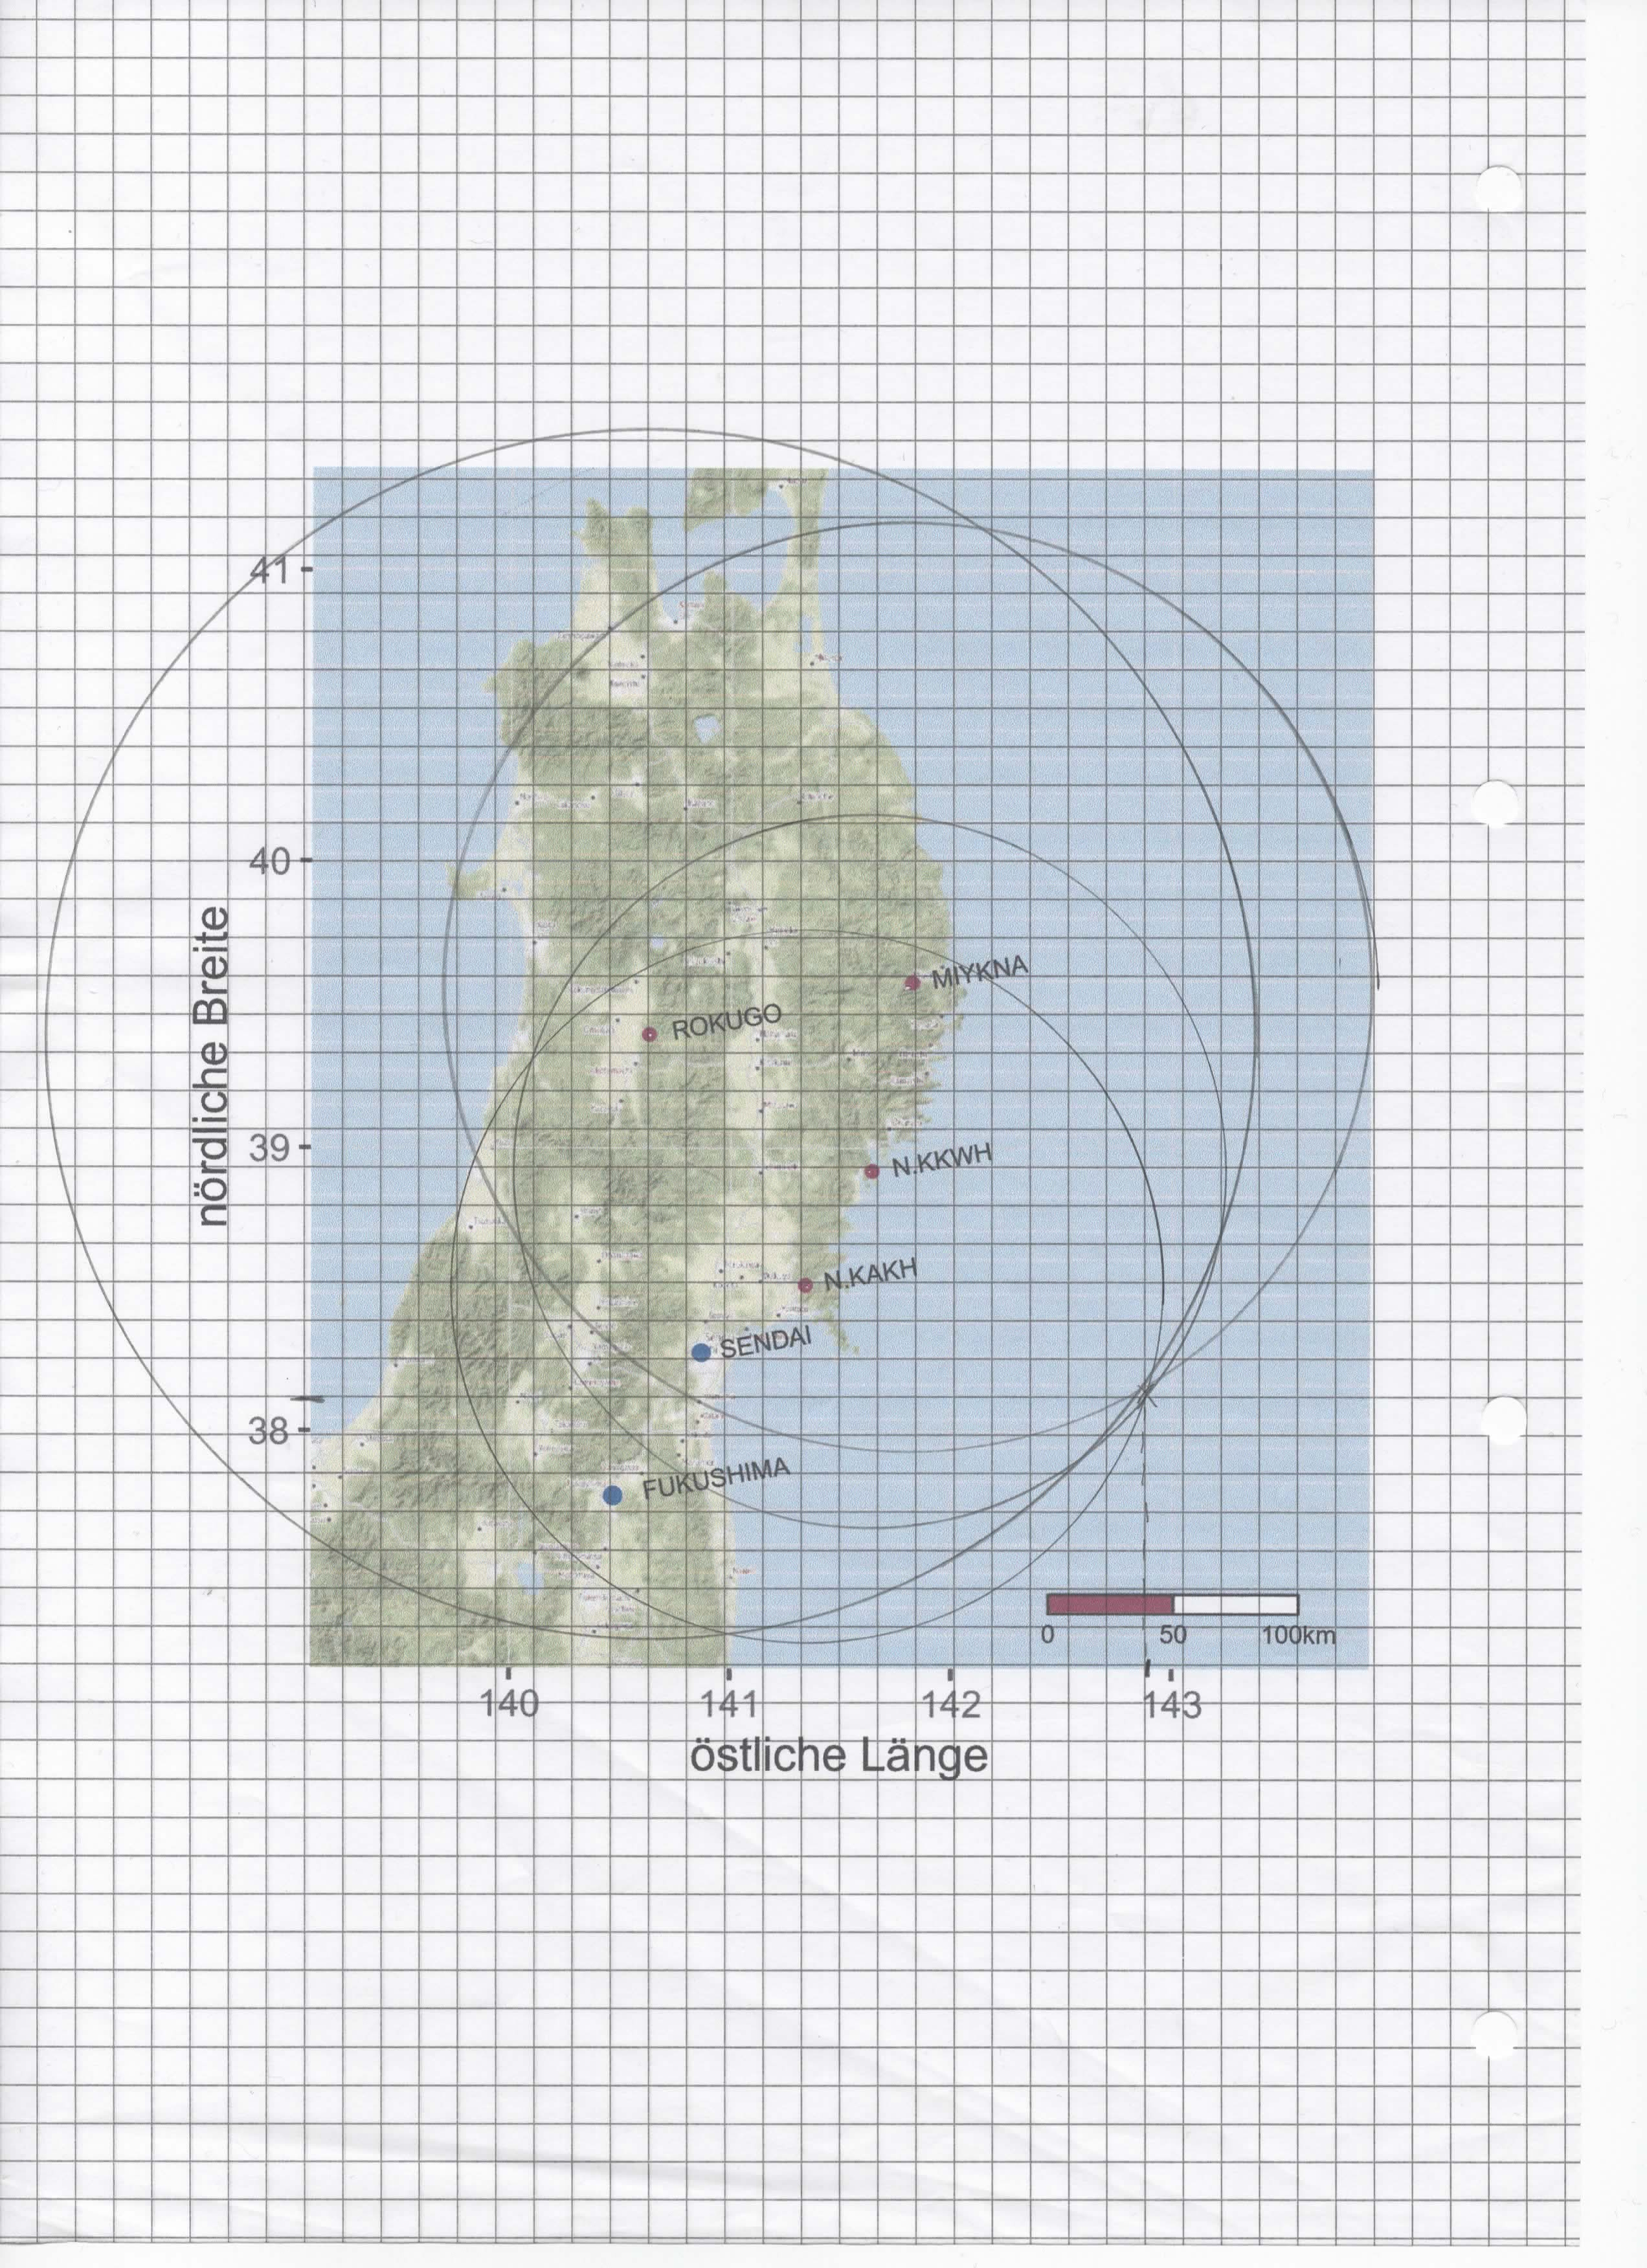
\includegraphics[scale=0.4]{PhotoScan.jpg}\\
	\textit{\textbf{M1 A1}}
\end{center}
\subsubsection*{2. Zeitpunkt berechnen}
Für die Berechnung des Zeitpunktes des Erdbebens verwende ich die Formel 
$t_0 = t_p - \frac{r}{v_p}$, 
wobei $t_p$ der Zeitpunkt des Eintreffens des Primärwellensignals ist. 
Ich berechne den Zeitpunkt aus den Werten $t_0$ aller vier Stationen und berechne den Mittelwert. 
In der folgenden Tabelle habe ich die Ergebnisse zusammengetragen.
\begin{center}
\begin{tabular}{l|l|l|l|l|l|l|l}
		   & $t_{p}$         & $t_s$         & $\Delta t$ & $r$      & $\frac{r}{v_p}$    & $\frac{r}{v_s}$    & $t_0$          \\\hline
	MIYKNA & 14:46:46,71 & 14:47:9,56  & 22,85   & 188,51 & 34,28 & 57,13 & 14:46:12,44 \\
	ROKUGO & 14:46:54,18 & 14:47:23,53 & 29,35   & 242,14 & 44,03 & 73,38 & 14:46:10,16 \\
	N.KKWH & 14:46:40,13 & 14:46:57,33 & 17,2    & 141,90 & 25,80 & 43,00 & 14:46:14,33 \\
	N.KAKH & 14:46:40,57 & 14:46:57,87 & 17,3    & 142,73 & 25,95 & 43,25 & 14:46:14,62 
\end{tabular}
\end{center}
Rechnet man jetzt den Mittelwert von den 4 $t_0$ Werten aus, kann man davon ausgehen, 
dass das Erdbeben um \textbf{14:46:12,89} stattgefunden hat.


\subsection*{Teilaufgabe b)}
Um das Verhältnis der Energien herauszufinden, drücke ich alle Energien über das gegebene Energieverhältnis durch $E_6$, der Energie eines Bebens der Stärke 6, aus. 
So kann man im Verhältnis der gesuchten Energien $E_6$ kürzen und bekommt die gesuchte Verhältniszahl.\\
Die Energie aller auftretenden Beben der Stärke 6-8 beschreibt die folgende Summe über die jeweiligen Energien multipliziert mit der Auftretenswahrscheinlichkeit pro Jahr. 
\begin{center}
$E_{alle} = 1 \cdot E_8 + 9 \cdot E_7 + 90 \cdot E_6$. 
\end{center}
Nachdem wir nun $E_{alle}$ haben, muss ich es nur noch mit $E_9$ (auch durch $E_6$ ausgedrückt) ins Verhältnis setzen, d.h.:
\begin{center}
$\frac{E_9}{E_{alle}} = \frac{E_6 \cdot 10^{\frac{3}{2} (9 - 6)}}{E_6 \cdot 10^{\frac{3}{2}(8-6)} + 9 \cdot E_6 \cdot 10^{\frac{3}{2}(7-6)} + 90 \cdot E_6}
= \frac{10^\frac{9}{2}}{10^3 + 0 \cdot 10^\frac{3}{2} + 90} \approx 23$
\end{center}
Das Beben hatte somit eine ca. \textbf{23-fach} höhere Energie.\\

\section*{Aufgabe 3}
\subsection*{Teilaufgaben a,b) Schwerpunktbahn und Drehfrequenz}
Die Bewegung der beiden Punkte kann man sich als Überlagerungen der Schwerpunktbewegung mit jeweils einer Kreisbewegung vorstellen, wobei die Schwerpunktbewegung in x-Richtung eine gleichförmige ist mit 
Anfangsposition 0 und in y-Richtung eine Überlagerung aus freiem Fall und gleichförmiger Bewegung mit Anfangsposition $y_0$.
\begin{center}
	$x_s (t)= v_{x0}\cdot t$ \\
	$y_s (t) = v_{y0}\cdot t + y_0 -0.5 g t^2$
\end{center}   
Die Überlagerten Kreisbewebungen sind
\begin{center}
	$x_p (t) = p \cdot (-\sin(\omega t))$ ; $x_q (t)= q \cdot (\sin(\omega t)) $\\
	$y_p (t) = p \cdot (\cos(\omega t))$ ; $y_q (t)= q \cdot (-\cos(\omega t)) $
\end{center} 
wobei $\omega = 2\pi f $ die Kreisfrequenz der Kreisbewegung mit der gesuchten Frequenz $f$ ist.\\
Zunächst rechne ich die Bewegung durch den freien Fall heraus, 
indem ich bei jedem $y$-Wert $0,5gt^2$ abziehe. Dadurch erhalte ich die folgenden Bahnkurven.
\begin{center}
	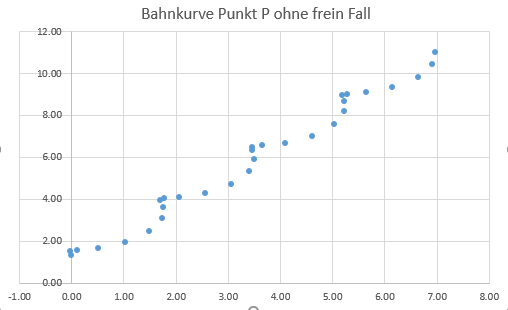
\includegraphics[scale=0.38]{Kurve-P-Punkt-ohne-freien-Fall.png}
	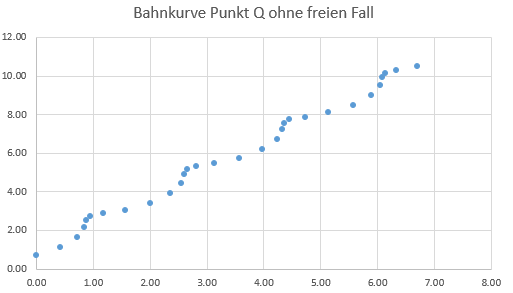
\includegraphics[scale=0.42]{Kurve-Q-Punkt-ohne-freien-Fall.png}
\end{center}
Um die Bewegung des Schwerpunktes herauszubekommen, zeichne ich die $x$-Koordinaten der Punkte P und Q Punkte sowie die $y$-Koordinaten der Punkte P und Q über der Zeit auf. 
\begin{center}
	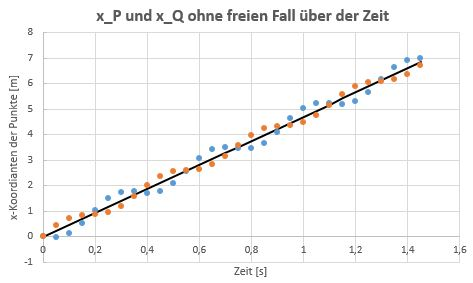
\includegraphics[scale=0.47]{x_s-ueber-Zeit.JPG}
	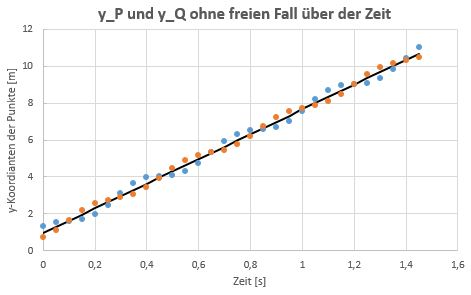
\includegraphics[scale=0.45]{y_s-ueber-Zeit.JPG}
\end{center}
Durch die Drehung des Schlägers streuen die Punkte jeweils um den Schwerpunkt. Ausgleichsgeraden durch die Punkte geben mir also die $x$-Bewegung und die $y$-Bewegung des Schwerpunktes.
Ich lese ab:
\begin{center}
	$x_s=4,72$m/s$\cdot t$ bzw. $ v_{xs} = 4,72$ m/s \\
	$y_s=6,71$m/s$\cdot t +0,95$m bzw. $ v_{ys} = 6,71$ m/s \\
\end{center}
Da nun die Abwurfgeschwindigkeiten bekannt sind, kann ich genauso wie ich den freien Fall abgezogen habe, nun auch den Anteil der geradlinigen Schwerpunkbewegung sowie die Position des Schwerpunktes zum Anfang ausrechnen.
Ich erhalte wunderschöne Kreisbahnen, aus denen ich die gefragten Größen $p$ und $q$ ablesen kann. 
\begin{center}
	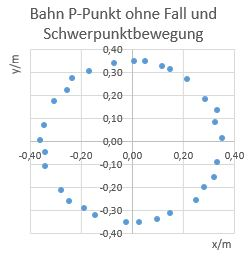
\includegraphics[scale=0.6]{Kreis-P.JPG}
	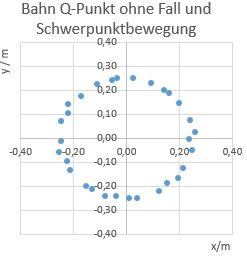
\includegraphics[scale=0.6]{Kreis-Q.JPG}
\end{center}
Ich finde für die Abstände der Punkte P und Q aus den Radien der Kreise die Werte 
\begin{center}
	$p=0,35$m und $q=0,25$m
\end{center}
Nun muss ich noch die Frequenz bestimmen. Dazu trage ich die Koordinaten der Punkte P und Q ohne die Schwerpunktbewegung gegen die Zeit auf 
und erhalte die erwarteten Sinusförmigen Kurven.   
\begin{center}
	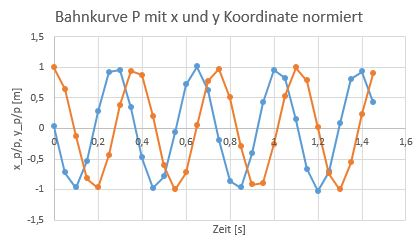
\includegraphics[scale=0.5]{Sinus-P.JPG}
	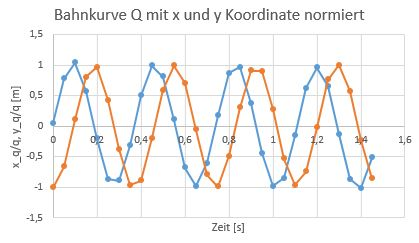
\includegraphics[scale=0.5]{Sinus-Q.JPG}
\end{center}
Aus diesen Kurven kann ich nun aus den Nulldurchgängen die Periodendauer und somit die 
Frequenz $f=1/T$ der Drehbewegung bestimmen. Ich lese für jeweils 3 Perioden die Zeit ab und erhalte als Mittelwert $3\cdot T=1,1$s.
Damit ergibt sich eine Frequenz von $2,7$Hz.\\
Bleibt -- auch wenn zu Beginn gefragt --  am Ende die Schwerpunktbahn, die sich aus den Werten für $v_{xs}$ und $v_{ys}$, den Anfangswerten und dem Beitrag des freien Falls berechnen lässt.
Mein Excel gibt mit die folgende Parabel-Kurve
\begin{center}
	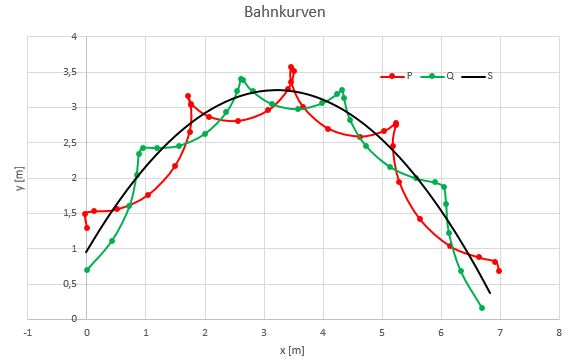
\includegraphics[scale=0.8]{Schwerpunktbahn.JPG}
\end{center}


\section*{Aufgabe 4}
\subsection*{Teilaufgabe a) Experiment - Messwerte}
Ich habe unsere Teekanne (ca. 1 Liter Fassungsvermögen) mit heißem Wasser aus dem Wasserkocher befüllt und anstelle des Deckels ein Thermometer aufgesetzt, welches zufälligerweise ideal passte. 
Das verwendete Heizungsventilthermometer hat einen Metallstab als Fühler, der ungefähr in der Mitte der Tekanne war. 
Zunächst alle 5 Minuten, später ungefähr alle 10 Minuten habe ich die Temperatur abgelesen. Die Ergebnisse stehen in den ersten zwei Spalten der folgenden Tabelle.\\ 
\newpage
\begin{tabular}{cccc}
	Zeit t {[}s{]} & Temp $\vartheta$ {[}°C{]}              & \begin{tabular}[c]{@{}l@{}}$\frac{\vartheta-\vartheta_u}{\vartheta_o-\vartheta_u}$\end{tabular} & $-\ln{\frac{\vartheta-\vartheta_U}{\vartheta_O-\vartheta_U}}$ \\\hline
	0              & 56,0 						  & 1,00                                                                 & 0,00     \\
	5              & 54,3                         & 0,95                                                                 & 0,05     \\
	10             & 53,0                         & 0,92                                                                 & 0,08     \\
	15             & 52,0                         & 0,89                                                                 & 0,11     \\
	20             & 50,0                         & 0,84                                                                 & 0,18     \\
	25             & 48,0                         & 0,78                                                                 & 0,24     \\
	30             & 47,0                         & 0,76                                                                 & 0,28     \\
	35             & 45,0                         & 0,70                                                                 & 0,35     \\
	40             & 44,0                         & 0,68                                                                 & 0,39     \\
	45             & 43,0                         & 0,65                                                                 & 0,43     \\
	50             & 42,3                         & 0,63                                                                 & 0,46     \\
	55             & 41,0                         & 0,59                                                                 & 0,52     \\
	60             & 40,0                         & 0,57                                                                 & 0,57     \\
	65             & 39,5                         & 0,55                                                                 & 0,59     \\
	70             & 39,0                         & 0,54                                                                 & 0,62     \\
	75             & 38,0                         & 0,51                                                                 & 0,67     \\
	80             & 37,5                         & 0,50                                                                 & 0,69     \\
	85             & 36,0                         & 0,46                                                                 & 0,78     \\
	90             & 36,0                         & 0,46                                                                 & 0,78     \\
	95             & 35,0                         & 0,43                                                                 & 0,84     \\
	100            & 34,0                         & 0,41                                                                 & 0,90     \\
	105            & 33,5                         & 0,39                                                                 & 0,94     \\
	110            & 33,0                         & 0,38                                                                 & 0,97     \\
	115            & 32,3                         & 0,36                                                                 & 1,02     \\
	120            & 32,0                         & 0,35                                                                 & 1,05     \\
	125            & 31,5                         & 0,34                                                                 & 1,09     \\
	130            & 31,0                         & 0,32                                                                 & 1,13     \\
	135            & 30,5                         & 0,31                                                                 & 1,17     \\
	140            & 30,0                         & 0,30                                                                 & 1,21     \\
	145            & 29,9                         & 0,29                                                                 & 1,22     \\
	150            & 29,7                         & 0,29                                                                 & 1,24     \\
	155            & 29,5                         & 0,28                                                                 & 1,26     \\
	160            & 28,7                         & 0,26                                                                 & 1,34     \\
	165            & 28,3                         & 0,25                                                                 & 1,38     \\
	170            & 28,0                         & 0,24                                                                 & 1,41     \\
	175            & 27,5                         & 0,23                                                                 & 1,47     \\
	180            & 27,3                         & 0,22                                                                 & 1,49     \\
	185            & 27,2                         & 0,22                                                                 & 1,51     \\
	190            & 26,5                         & 0,20                                                                 & 1,60 
\end{tabular}
\begin{tabular}{cccc}
	Zeit t {[}s{]} & Temp $\vartheta$ {[}°C{]}              & \begin{tabular}[c]{@{}l@{}}$\frac{\vartheta-\vartheta_u}{\vartheta_o-\vartheta_u}$\end{tabular} & $-\ln{\frac{\vartheta-\vartheta_U}{\vartheta_O-\vartheta_U}}$ \\\hline
	200            & 25,9                         & 0,19                                                                 & 1,68     \\
	218            & 24,5                         & 0,15                                                                 & 1,91     \\
	228            & 24,1                         & 0,14                                                                 & 1,98     \\
	238            & 24,0                         & 0,14                                                                 & 2,00     \\
	248            & 23,7                         & 0,13                                                                 & 2,06     \\
	265            & 22,3                         & 0,09                                                                 & 2,42     \\
	275            & 22,1                         & 0,08                                                                 & 2,48     \\
	286            & 22,0                         & 0,08                                                                 & 2,51     \\
	297            & 21,9                         & 0,08                                                                 & 2,55     \\
	308            & 21,5                         & 0,07                                                                 & 2,69     \\
	319            & 20,5                         & 0,04                                                                 & 3,21     \\
	330            & 20,3                         & 0,04                                                                 & 3,35     \\
	341            & 20,1                         & 0,03                                                                 & 3,52     \\
	352            & 20,0                         & 0,03                                                                 & 3,61     \\
	363            & 19,9                         & 0,02                                                                 & 3,72     \\
	374            & 19,8                         & 0,02                                                                 & 3,83     \\
	385            & 19,8                         & 0,02                                                                 & 3,83     
\end{tabular}
\newpage
Die Abkühlkurve meines Experiments sieht wie folgt aus. 
\begin{center}
	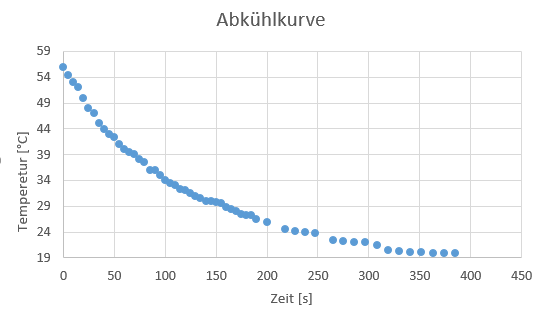
\includegraphics[scale=0.6]{Graph1.png}
\end{center}


\subsection*{Teilaufgabe b) - Bestimmung Zeitkonstante}
Zunächst will ich zeigen, dass die gewonnene Abkühlkurve gemäß der Newtonschon Formel 
\begin{center}
	$\vartheta (t) = \vartheta_u + (\vartheta_o - \vartheta_u) \cdot e^{-t/\tau}$ 
\end{center}
verläuft. Dazu forme ich die Gleichung wie folgt um
\begin{center}
	$\frac{\vartheta (t) - \vartheta_u}{\vartheta_o - \vartheta_u} = e^{-t/\tau}$ 
\end{center}
Ich nehme den Logarithmus auf beiden Seiten der Gleichung und erhalte eine Geradengleichung, 
aus deren Steigung sich die Abkühlkonstante $\tau$ berechnen lässt.
\begin{center}
	$-\ln{\frac{\vartheta (t) - \vartheta_u}{\vartheta_o - \vartheta_u}} = \frac{1}{\tau}\cdot t$ 
\end{center}
Die Ergebnisse des linken Terms habe ich ebenfalls in der obigen Tabelle eingetragen. 
Wie man in der folgenden Graphik sieht, liegen die Messwerte tatsächlich auf einer Geraden. Somit habe ich gezeigt, dass der Abkühlprozess tatsächlich dem Newtonschon Gesetz folgt.  
\begin{center}
	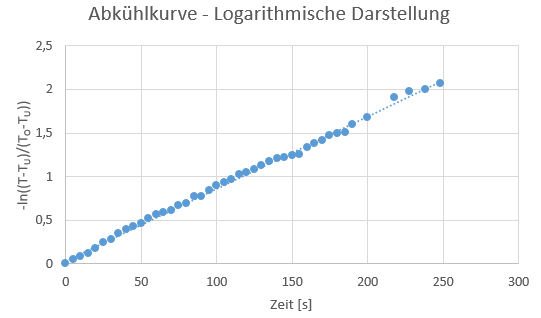
\includegraphics[scale=0.6]{Graph2.png}
\end{center}
Die Steigung der Geraden lese ich ab mit$\frac{2,2}{250}\cdot\frac{1}{s}=\frac{0,0088}{s}$.
Der Kehrwert ist die gesuchte Abkühlkonstante $\tau = 113,6 s$.
\subsection*{Teilaufgabe c) - Zubereitung Grüner Tee}
Ich verwende das Newtonsche Abkühlungsgesetz, diesmal mit $\vartheta_o=100^\circ C$.
\begin{center}
	$70^\circ C = \vartheta (t) = \vartheta_u + (100^\circ C - \vartheta_u ) \cdot e^{-t/\tau}$ 
\end{center}
Es ergibt sich mit dem oben bestimmten Wert für $\tau$ und $\vartheta (t) = 70^\circ C$
\begin{center}
	$t=-\tau \ln{\frac{\vartheta (t) - \vartheta_u}{ 100^\circ C - \vartheta_u}} \approx 53 s$
\end{center}
Dieses Ergebnis ist wie in der Aufgabe beschrieben eher ungenau, da das Newtonsche Abkühlgesetz nur für kleine Temperaturdifferenzen gilt und 
die Größe $\tau$ sicherlich auch eine gewisse Abhängigkeit von der Temperatur hat.\\In Lehrbuecherns findet man z.B. eine inverse Abh\"angigkeit von der W\"arme-kapazit\"at des Wassers.
Da das Wasser knapp unter dem Siedepunkt stärker verdampft als bei kleinen Temperaturen, entzieht die Verdampfungswärme dem Teewasser bei den hohen Temperaturen zusätzliche Energie, 
was ein schnelleres Erkalten des Teewassers erwarten lässt. 
Die Newtonsche Abkühlungskurve beschreibt ja lediglich den Wärmeübergang durch Wärmeleitung ins Gefäß und die umgebende Luft durch die Abstrahlung. 
Energieänderung durch Verdampfen ist nicht enthalten.      
\end{document}
